\documentclass[final]{article}
\usepackage[a0paper,portrait,margin=20mm]{geometry}

\usepackage{iftex}
\ifPDFTeX
  \usepackage[T1]{fontenc}
  \usepackage[utf8]{inputenc}
  \usepackage[scaled]{helvet}
  \renewcommand{\familydefault}{\sfdefault}
\else
  \usepackage{fontspec}
  \setmainfont{Arial}
  \setsansfont{Arial}
\fi

\usepackage[spanish]{babel}
\usepackage{graphicx}
\usepackage[table]{xcolor}
\usepackage{multicol}
\usepackage{tabularx}
\usepackage{array}
\usepackage{float}
\usepackage{booktabs}
\usepackage{amsmath}
\usepackage{amssymb}
\usepackage{tikz}
\usetikzlibrary{positioning, arrows.meta}
\usepackage{caption}
\usepackage[numbers]{natbib}
\usepackage{url}
\captionsetup{font={large},labelfont=bf,skip=1pt}
\graphicspath{{../figures/}{../figures/logos/}}
\providecommand{\newblock}{\relax}
\providecommand{\BIBentrySTDinterwordspacing}{\spaceskip=0pt\relax}
\providecommand{\BIBentryALTinterwordstretchfactor}{4}
\providecommand{\BIBentryALTinterwordspacing}{\spaceskip=\fontdimen2\font plus
\BIBentryALTinterwordstretchfactor\fontdimen3\font minus \fontdimen4\font\relax}

\definecolor{sectionred}{HTML}{000000}
\pagestyle{empty}
\setlength{\parindent}{0pt}
\setlength{\parskip}{0.14\baselineskip}
\setlength{\columnsep}{16mm}
\setlength{\columnseprule}{0pt}


\newcommand{\posterlogo}[2]{%
  \IfFileExists{#1}{\includegraphics[height=60mm,width=0.25\textwidth,keepaspectratio]{#1}}{%
    \IfFileExists{logos/#1}{\includegraphics[height=60mm,width=0.25\textwidth,keepaspectratio]{logos/#1}}{\fbox{\parbox[c][80mm][c]{0.25\textwidth}{\centering\large #2}}}%
  }%
}

\newcommand{\sectiontitle}[1]{\vspace{4.2mm}{\color{sectionred}\bfseries\fontsize{21}{24}\selectfont #1}\par\vspace{0.8mm}{\color{sectionred}\rule{\linewidth}{1.0pt}}\par\vspace{1.4mm}}

\newcommand{\postersubtitle}[1]{\vspace{2.0mm}{\bfseries\fontsize{16.8}{19}\selectfont #1}\par\vspace{0.45mm}}

\begin{document}
\begin{center}
  \begin{tabularx}{\textwidth}{@{}>{\raggedright\arraybackslash}X>{\centering\arraybackslash}X>{\raggedleft\arraybackslash}X@{}}
    \posterlogo{../figures/logo_UNA.png}{Logo UNA} &
    \posterlogo{../figures/logo_JJII.png}{Logo JJI+i} &
    \posterlogo{../figures/fiuna_logo.png}{Logo FIUNA}
  \end{tabularx}

  \vspace{2mm}
  {\bfseries\fontsize{34}{39}\selectfont Desarrollo de un Prototipo de Procesamiento Local para la Detección, Clasificación y Análisis Predictivo de Manchas Solares mediante Visión Computacional e Inteligencia Artificial\par}

  \vspace{2mm}
  {\fontsize{19}{23}\selectfont Benítez, Carlos\textsuperscript{1}; Cabral, Juan\textsuperscript{2}; Stalder, Diego\textsuperscript{1}; Gómez, José María\textsuperscript{2}; Schaerer, Christian\textsuperscript{2}; Núñez, Jesús\textsuperscript{1}\par}
  \vspace{1.5mm}
  {\fontsize{17}{21}\selectfont \textsuperscript{1}Facultad de Ingeniería, Universidad Nacional de Asunción; \textsuperscript{2}Facultad Politécnica, Universidad Nacional de Asunción\par}
  \vspace{2mm}
  {\fontsize{16}{19}\selectfont \textbf{Palabras clave:} manchas solares, visión computacional, inteligencia artificial, Zurich--McIntosh, PVL--Kalman, DMD, YOLO26n, ConvNeXtV2a, Raspberry Pi 5\par}
\end{center}

\vspace{1mm}\noindent{\color{sectionred}\rule{\textwidth}{1.8pt}}\vspace{1mm}

{\fontsize{15.8}{18.8}\selectfont
\begin{multicols}{2}

\sectiontitle{INTRODUCCIÓN}
El análisis automático de manchas solares es relevante para el monitoreo operativo de la actividad fotosférica y para interpretar condiciones de clima espacial que pueden afectar instrumentación y sistemas de comunicación. En observatorios terrestres y académicos, la adquisición de imágenes, el registro de metadatos, la identificación de grupos solares y la clasificación Zurich--McIntosh suelen ejecutarse como tareas separadas y manuales, reduciendo la trazabilidad entre observación original, recortes, etiquetas y consulta posterior. Este trabajo propone una cadena integrada de adquisición en luz blanca, procesamiento local, inferencia con inteligencia artificial, sincronización de datos y visualización web, orientada a observatorios con recursos computacionales y conectividad variables.

\sectiontitle{ARQUITECTURA}
\begin{figure}[H]
    \centering
    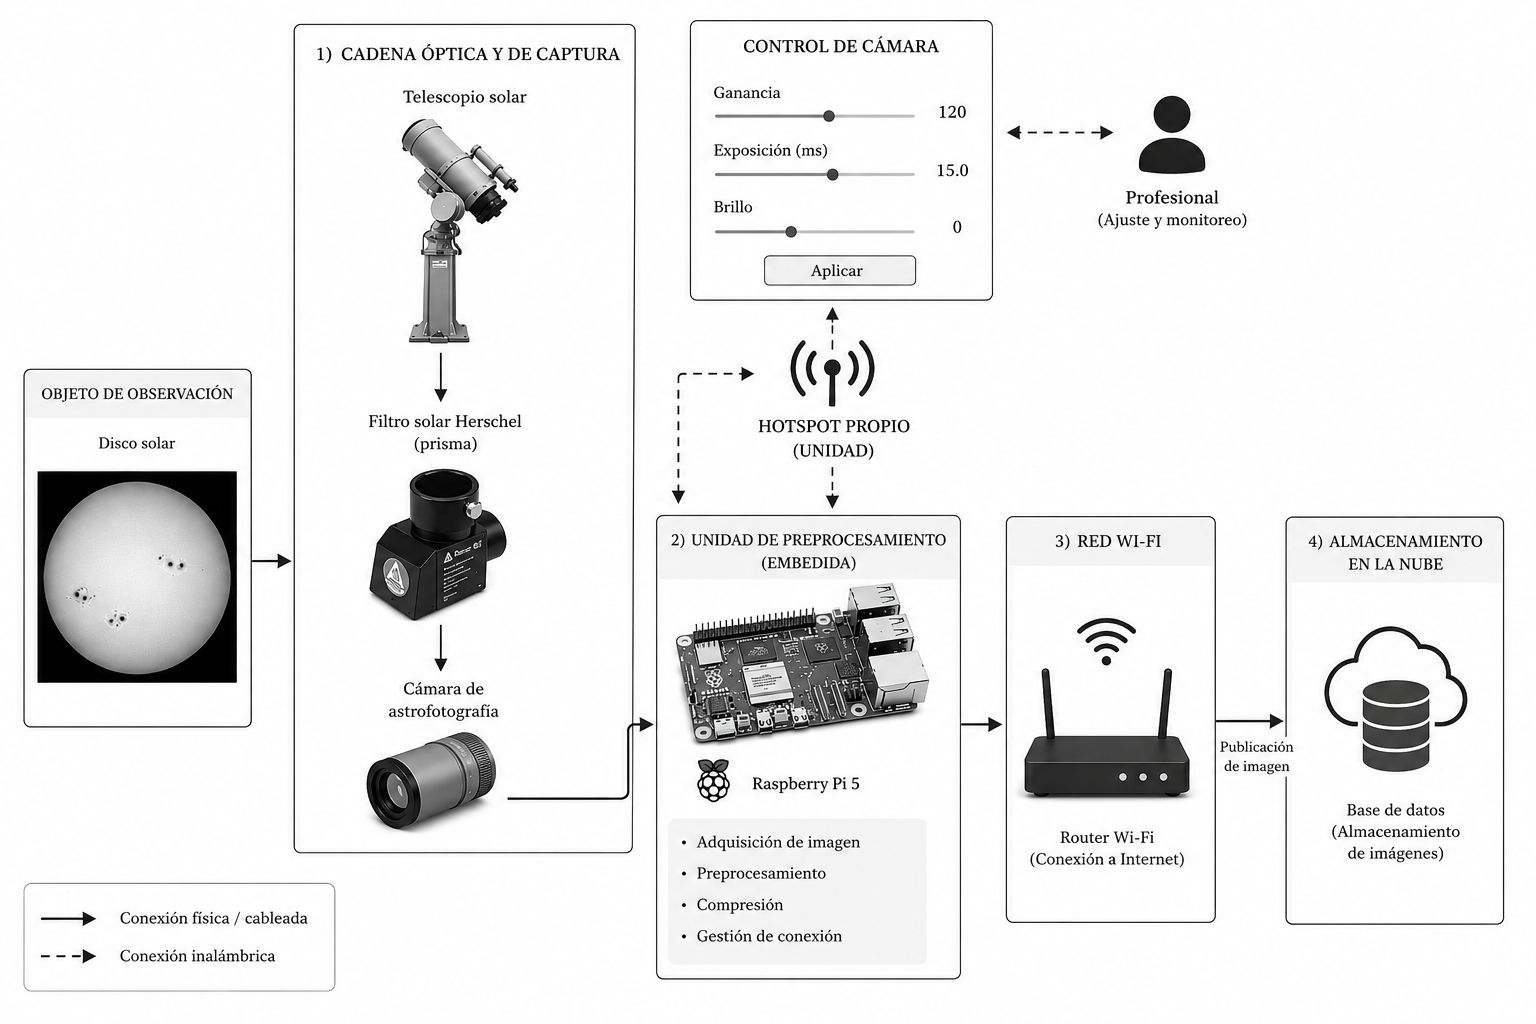
\includegraphics[width=0.48\linewidth]{hw/module.png}
    \caption{Módulo de observación solar implementado.}
\end{figure}

El sistema emplea cámara monocromática ZWO ASI174MM Mini, cuña de Herschel, telescopio refractor Vixen de $D=60$ mm y $F=420$ mm, y Raspberry Pi 5 con refrigeración activa como nodo de borde. La base de datos combina imágenes SDO/HMI, reportes NOAA SRS y observaciones propias; Supabase desacopla captura, consulta e inferencia.

\begin{figure}[H]
    \centering
    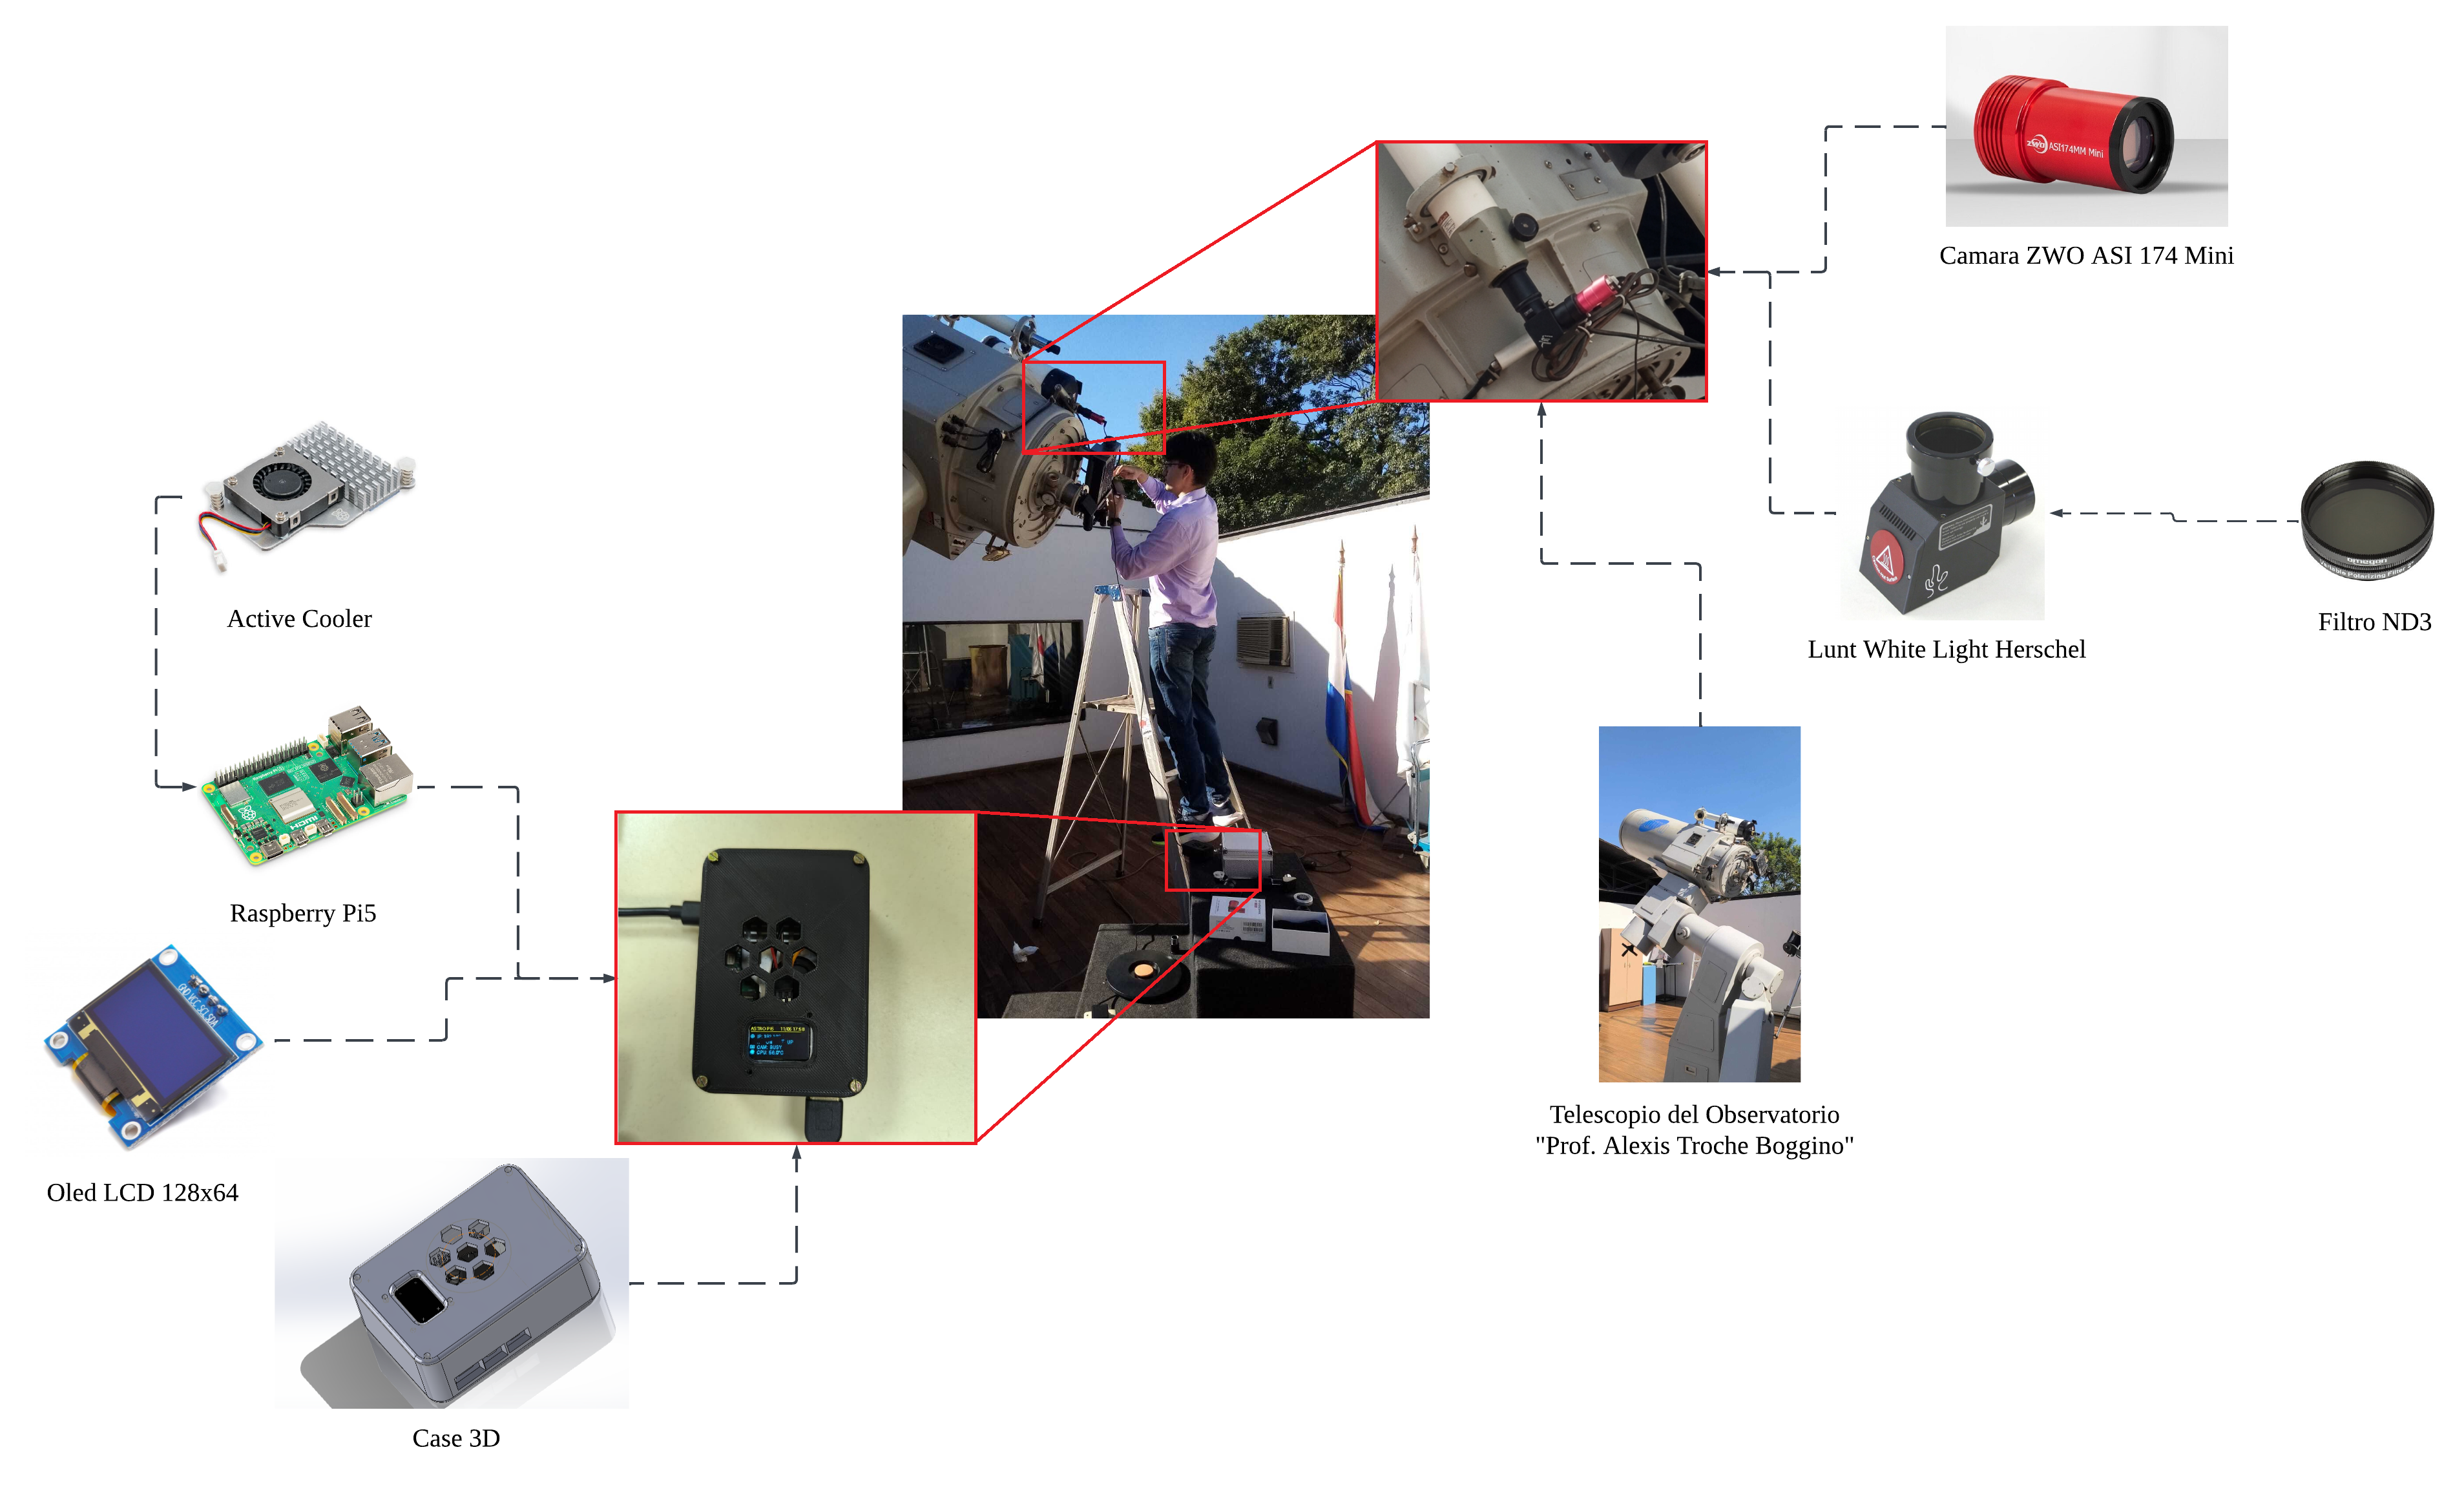
\includegraphics[width=0.80\linewidth]{hw/hw_diagram.png}
    \caption{Flujo físico del hardware de captura, procesamiento local y publicación.}
\end{figure}

\sectiontitle{FORMULACIÓN IA}
La cadena utiliza YOLO26n para estimar cajas $b_i=(x_i,y_i,w_i,h_i)$ y ConvNeXtV2a para inferir salidas jerárquicas $Z$, $P$ y $C$:
\[
\mathbf{f}=\mathrm{GAP}(\mathrm{ConvNeXtV2}(x)),\quad
\hat{\mathbf{p}}_Z=\mathrm{softmax}(g_Z(\mathbf{f})),
\]
\[
\hat{\mathbf{p}}_P,\hat{\mathbf{p}}_C=\mathrm{softmax}(g([\mathbf{f};\hat{\mathbf{p}}_Z])).
\]
La recomendación se restringe al espacio Zurich--McIntosh válido:
\[
P_{\mathrm{rec}}=\frac{P(Z\mid x)P(P\mid x)P(C\mid x)M_{ZPC}}
{\sum_{z,p,c}P(z\mid x)P(p\mid x)P(c\mid x)M_{zpc}}.
\]
Para predicción se combinan PVL--Kalman,
\[
K_k=P_k^-(P_k^-+R_k)^{-1},\quad \hat{s}_k=\hat{s}_k^-+K_k(z_k-\hat{s}_k^-),
\]
y DMD, con evolución latitudinal $\mathbf{x}_{k+1}\approx\mathbf{A}\mathbf{x}_k$.

\begin{figure}[H]
    \centering
    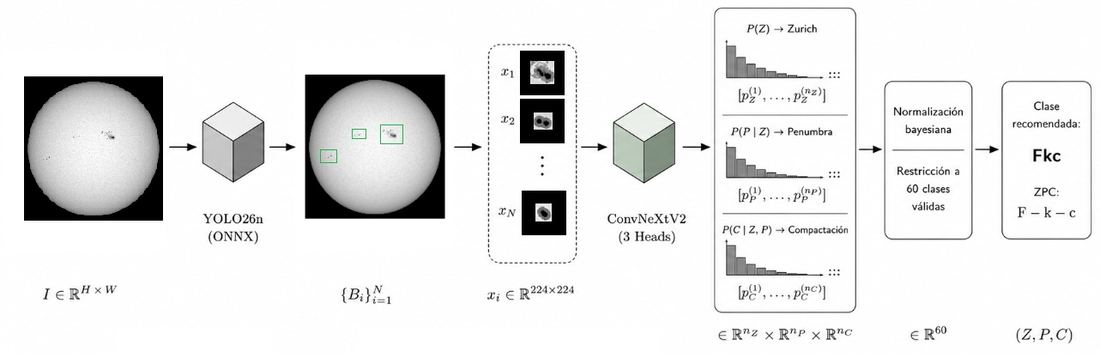
\includegraphics[width=0.80\linewidth]{sys/img_pipe.jpg}
    \caption{Cadena de procesamiento de imágenes solares.}
\end{figure}

\sectiontitle{RESULTADOS}
\postersubtitle{Clasificación automática}
YOLO26n localiza grupos solares y ConvNeXtV2a estima los componentes $Z$, $P$ y $C$ manteniendo una salida jerárquica e interpretable.
\begin{figure}[H]
    \centering
    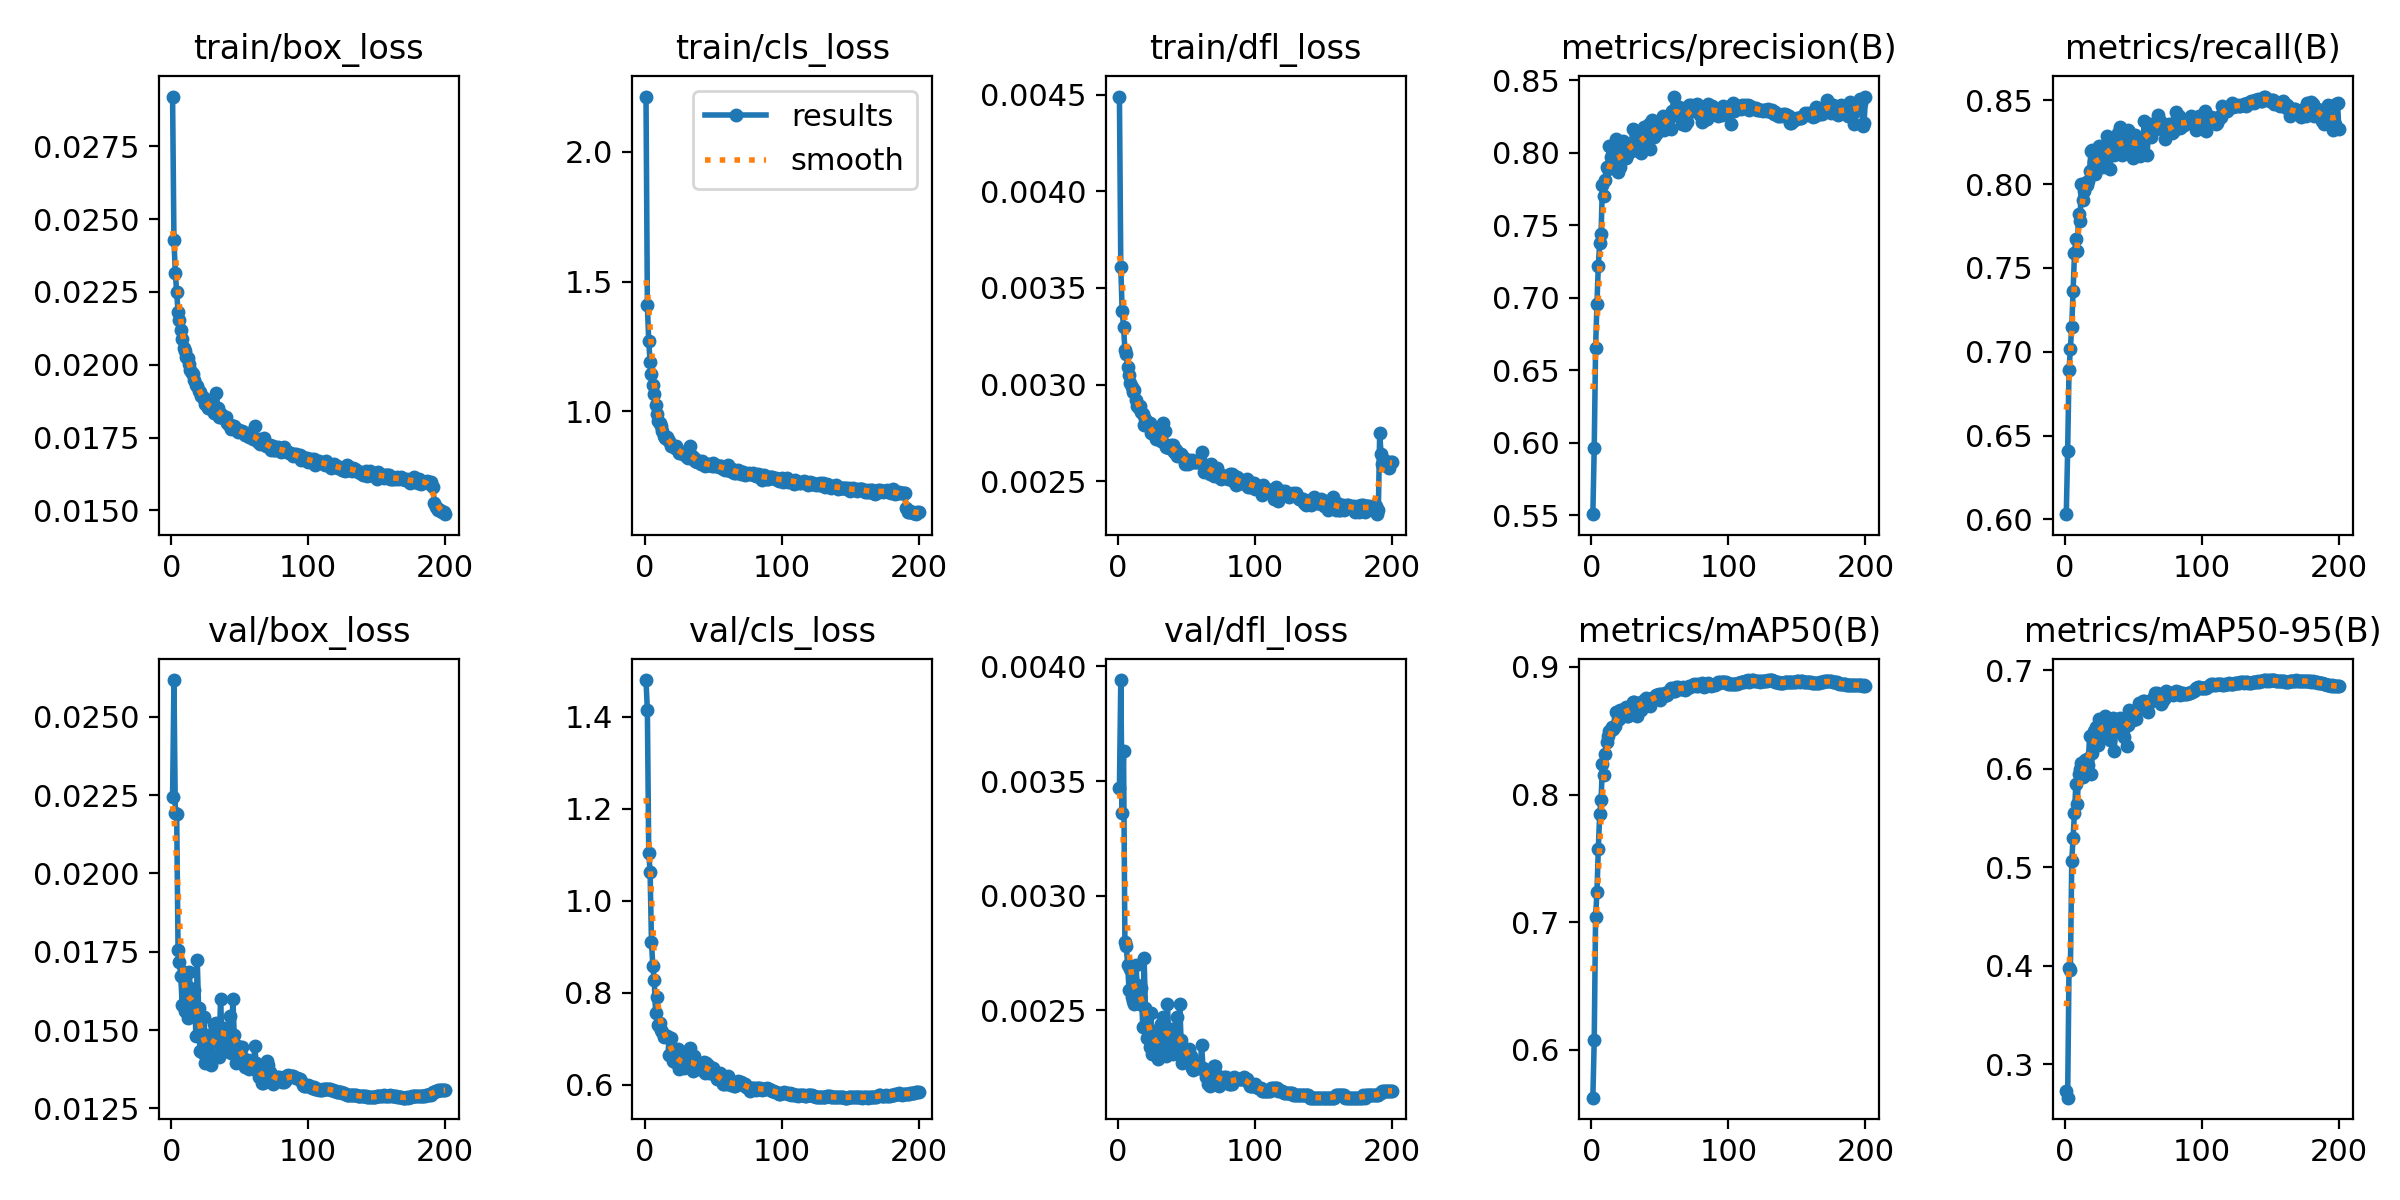
\includegraphics[width=0.64\linewidth]{ml/yolo_results.png}
    \caption{Agrupamiento de regiones activas mediante YOLO26n.}
\end{figure}

\begin{figure}[H]
    \centering
    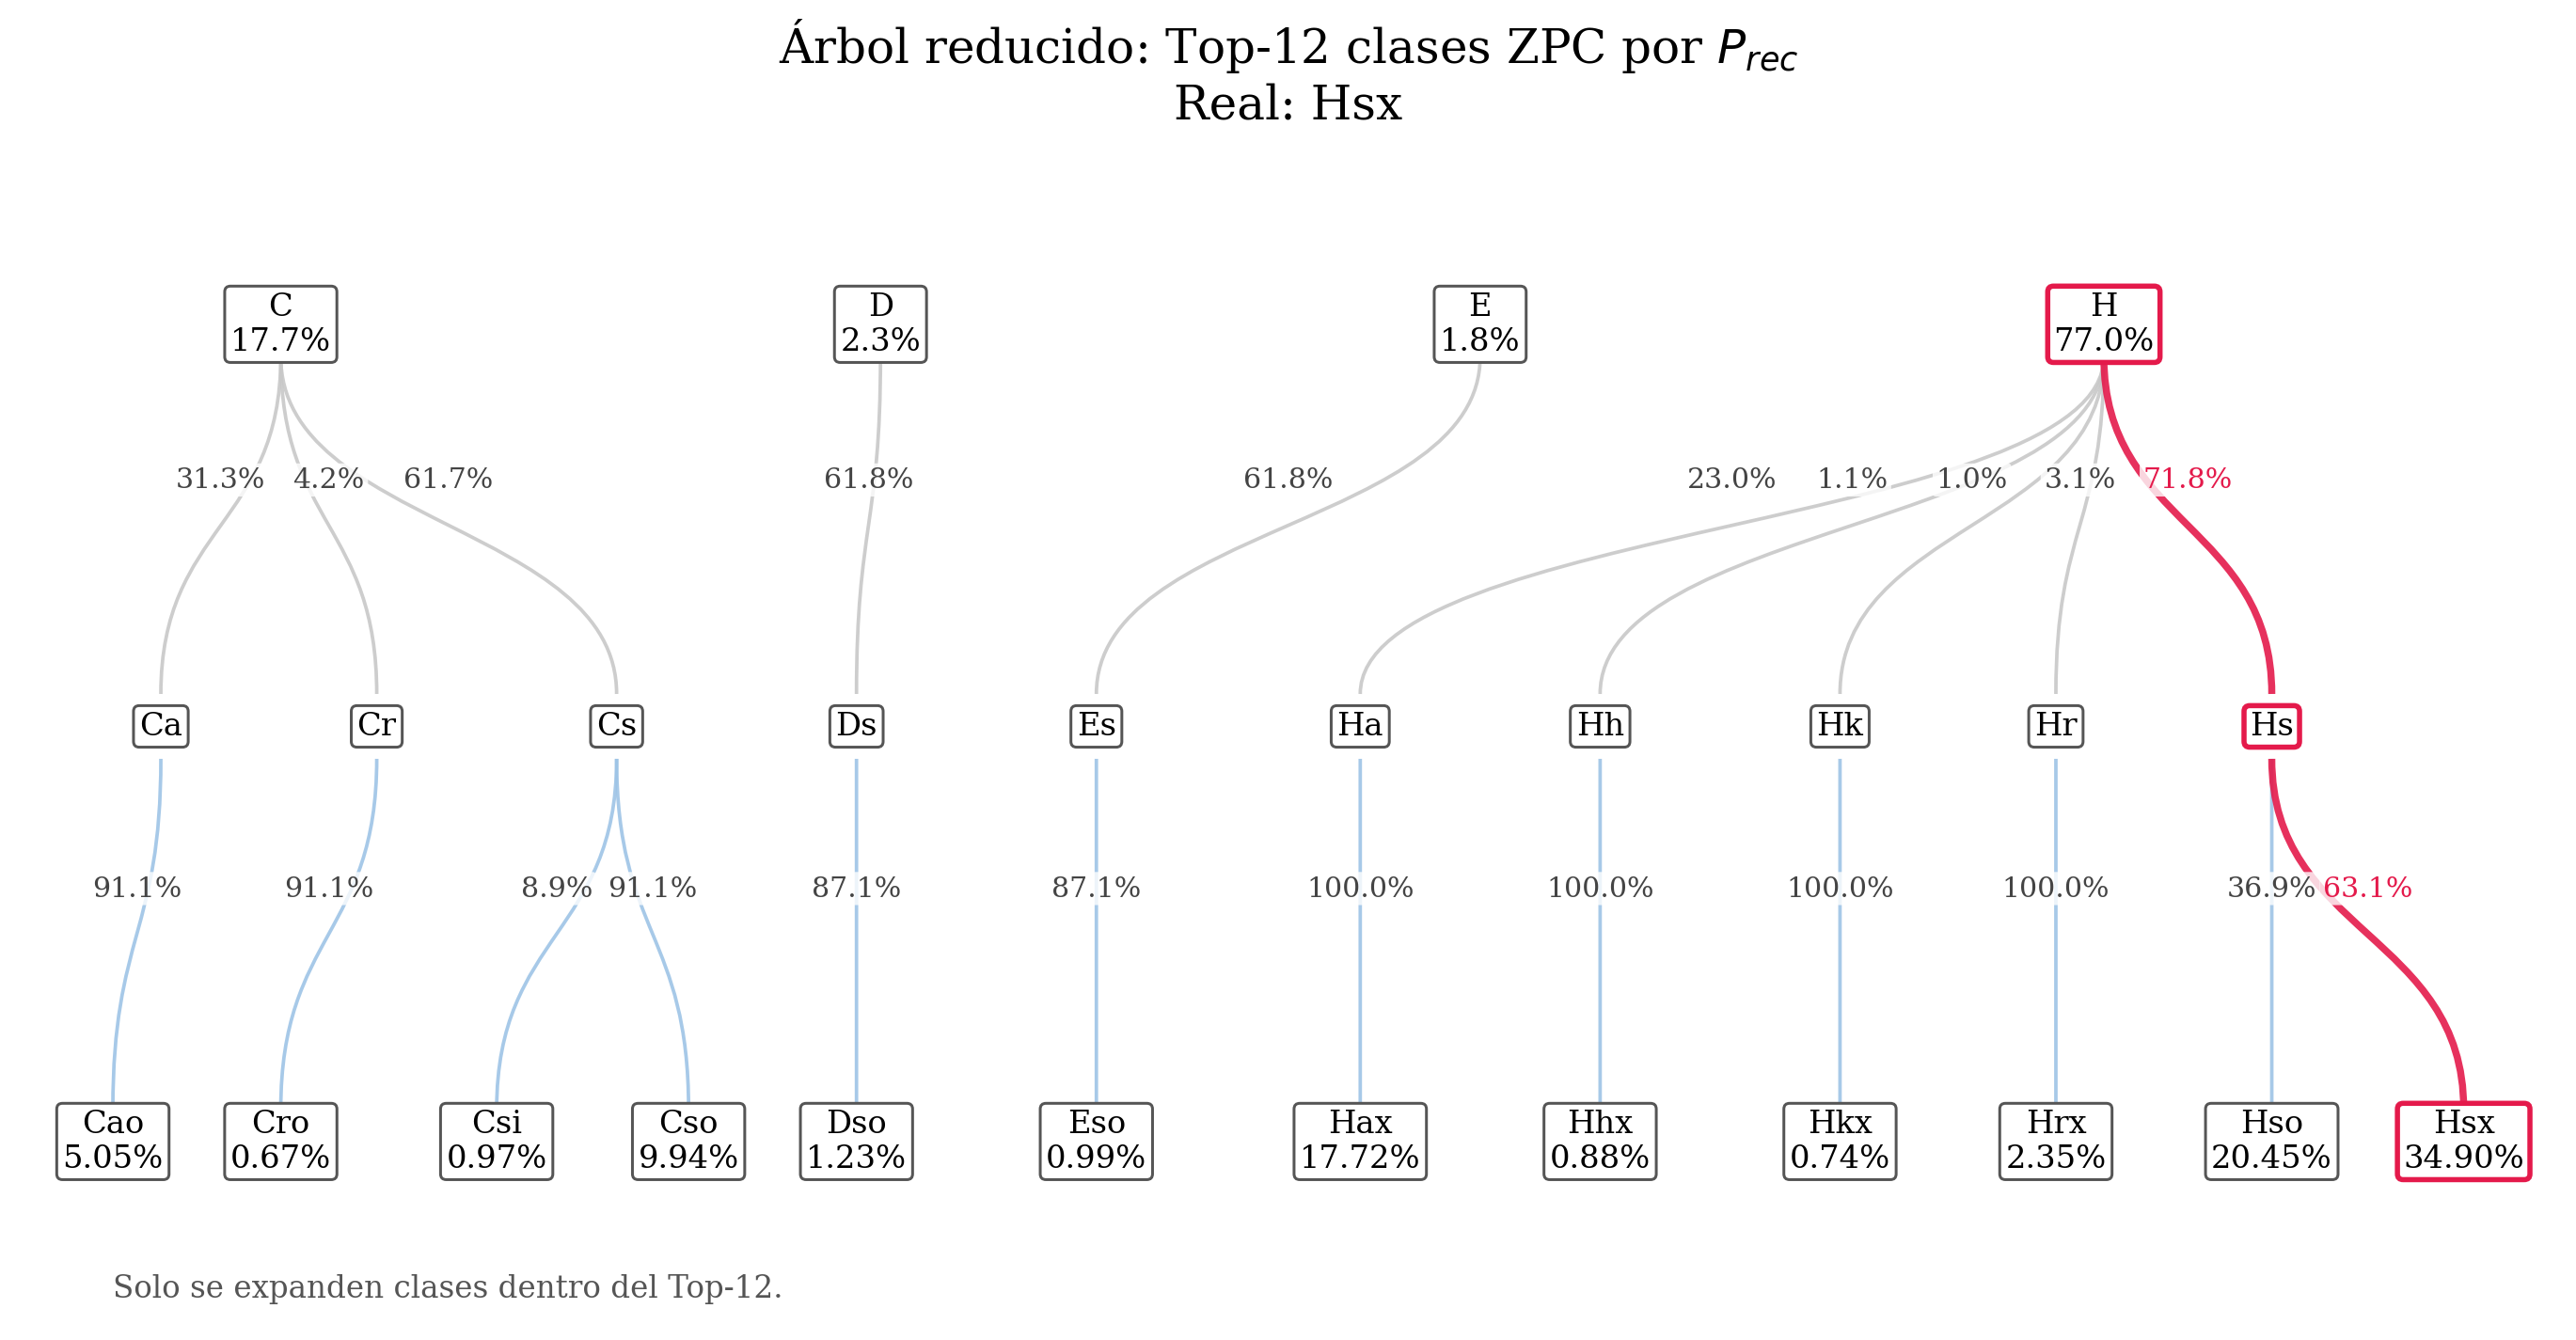
\includegraphics[width=0.46\linewidth]{ml/top12_tree.png}
    \caption{Recomendación jerárquica Zurich--McIntosh con combinaciones válidas.}
\end{figure}

\begin{center}
\begin{tabular}{lccc}
\toprule
\textbf{Salida} & \textbf{Precisión} & \textbf{Recall} & \textbf{F1} \\
\midrule
Z & 0.68 & 0.63 & 0.65 \\
P & 0.66 & 0.61 & 0.63 \\
C & 0.74 & 0.69 & 0.71 \\
\bottomrule
\end{tabular}
\end{center}

\columnbreak

\postersubtitle{Predicción solar}
PVL--Kalman resume la amplitud temporal del SSN, mientras DMD reconstruye la distribución latitudinal tipo Spörer.
\begin{figure}[H]
    \centering
    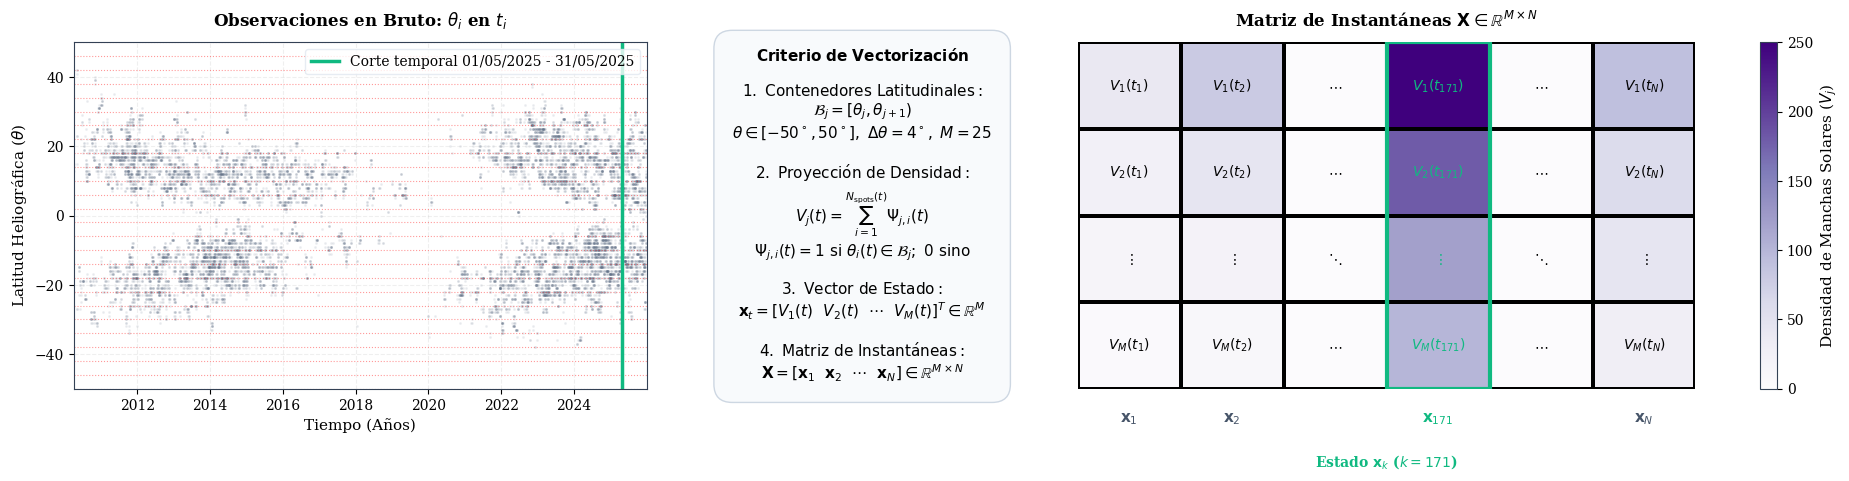
\includegraphics[width=0.88\linewidth]{dmd/discretizacion.png}
    \caption{Discretización latitudinal del diagrama de Spörer.}
\end{figure}
\begin{figure}[H]
    \centering
    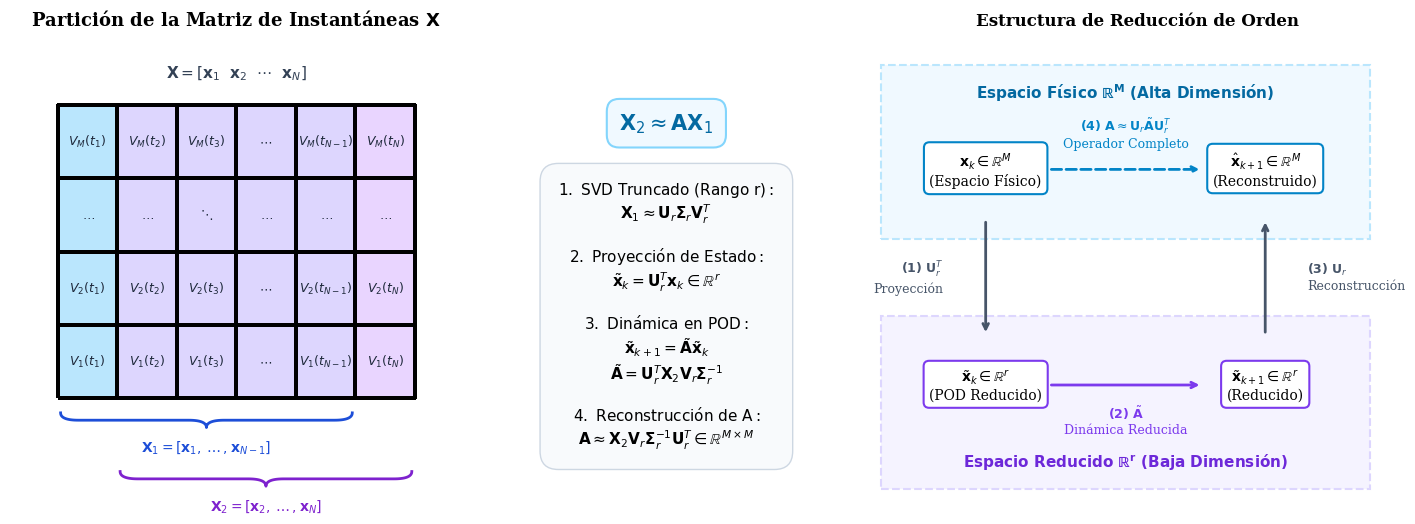
\includegraphics[width=0.88\linewidth]{dmd/dmd.png}
    \caption{Operador dinámico empleado para la reconstrucción DMD--Spörer.}
\end{figure}
\begin{figure}[H]
    \centering
    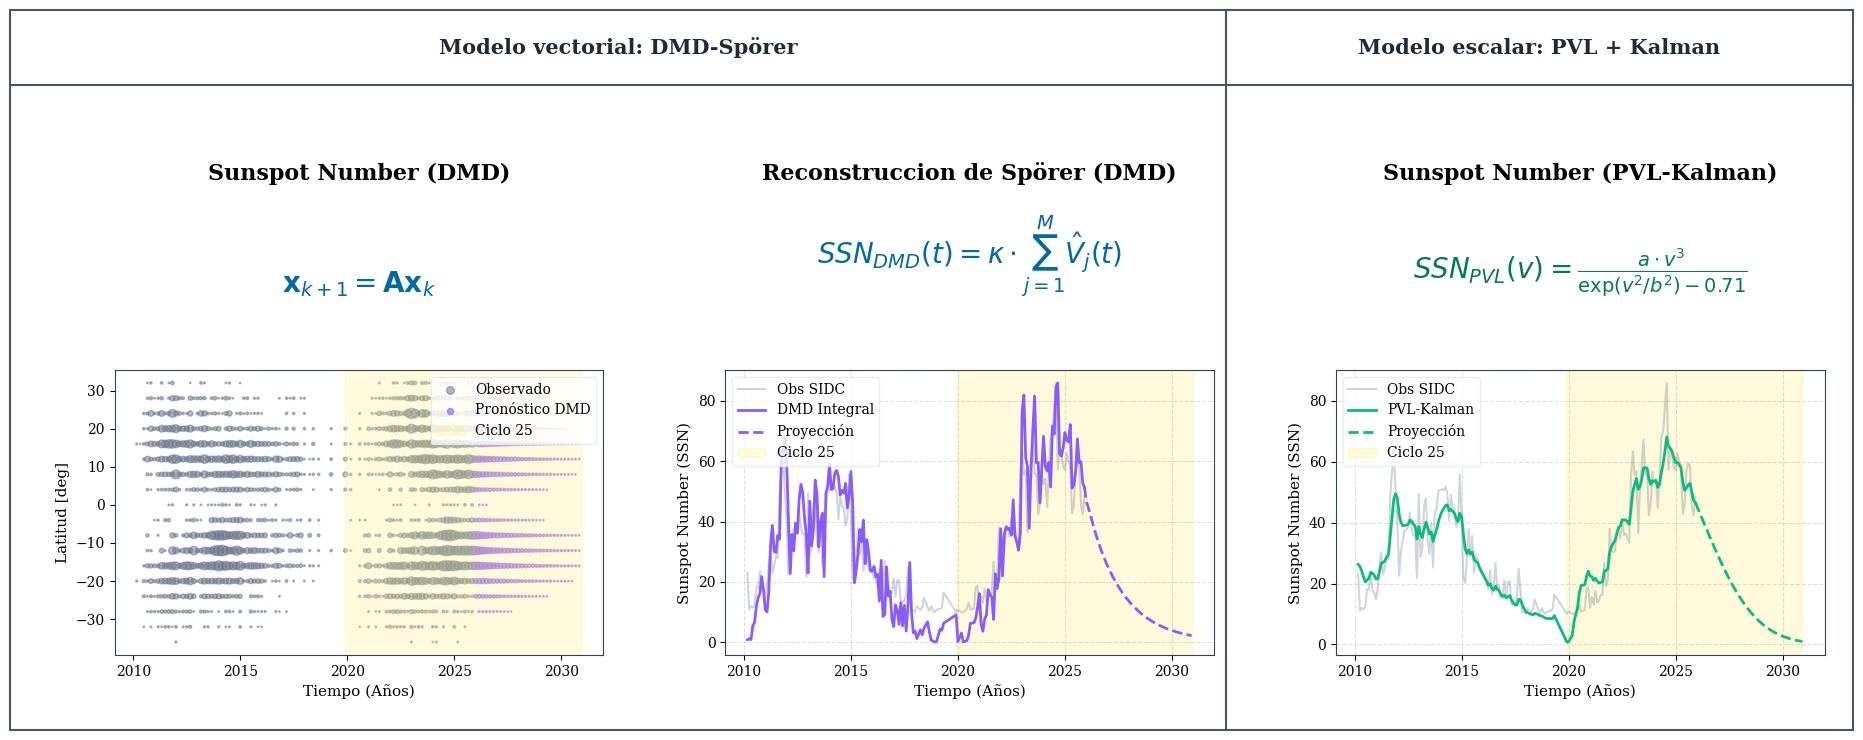
\includegraphics[width=0.88\linewidth]{dmd/model_results.png}
    \caption{Comparación visual del modelo vectorial DMD y el modelo escalar PVL--Kalman.}
\end{figure}

\begin{center}
\begin{tabular}{lcc}
\toprule
\textbf{Métrica} & \textbf{$\mathrm{SSN}_{\mathrm{PVLK}}$} & \textbf{$\mathrm{SSN}_{\mathrm{DMD}}$} \\
\midrule
MAE & 15.31 & 15.22 \\
RMSE & 22.02 & 20.30 \\
MAPE & 33.27\% & 32.54\% \\
$R^2$ & 0.8173 & 0.8449 \\
\bottomrule
\end{tabular}
\end{center}

\begin{center}
\begin{tabular}{lc}
\toprule
\textbf{DMD--Spörer} & \textbf{Valor} \\
\midrule
$E_F$ & 0.4087 \\
$\rho_{ST}$ & 0.9126 \\
MLCE & $1.25^{\circ}$ \\
\bottomrule
\end{tabular}
\end{center}

\postersubtitle{Integración con plataforma web}
La captura real del 2026-05-05 verificó adquisición, guardado local, preprocesamiento y sincronización. La operación representativa registró 420 ms para captura individual, 180 ms para guardado local, 1350 ms para preprocesamiento, 3800 ms por imagen para sincronización, 38\% de CPU media y 57 $^{\circ}$C tras 25 minutos, sin reinicios ni reducción térmica perceptible.

\begin{figure}[H]
    \centering
    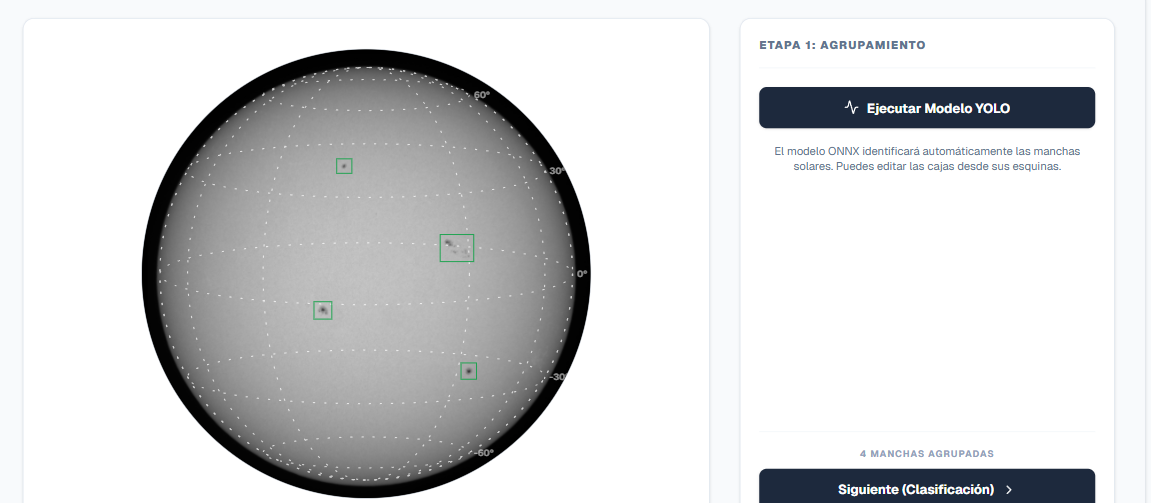
\includegraphics[width=0.58\linewidth]{web/yolo.png}
    \caption{Inferencia local en navegador mediante YOLO26n.}
\end{figure}
\begin{figure}[H]
    \centering
    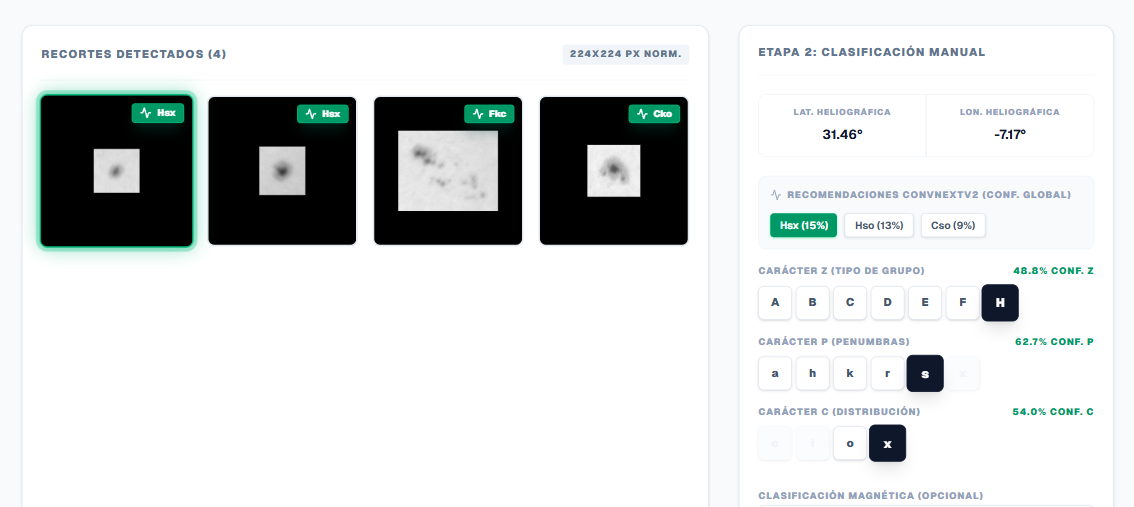
\includegraphics[width=0.58\linewidth]{web/convnext.png}
    \caption{Clasificación morfológica local mediante ConvNeXtV2a.}
\end{figure}
\begin{center}
    
\includegraphics[width=0.16\linewidth]{qr/web.png}\par
    {\fontsize{10.2}{11.5}\selectfont Código QR de acceso a la plataforma web del sistema.}
\end{center}

\sectiontitle{CONCLUSIONES}
La contribución principal del prototipo es una arquitectura trazable que conecta adquisición, metadatos, inferencia, visualización y análisis temporal en una misma cadena operativa. El enfoque jerárquico respeta la taxonomía Zurich--McIntosh y evita una clasificación plana de combinaciones morfológicas, mientras que PVL--Kalman y DMD aportan lecturas complementarias del ciclo solar: amplitud global y migración latitudinal. La ejecución local con modelos ONNX refuerza la portabilidad del sistema y lo vuelve adecuado para observatorios académicos con conectividad limitada.

\sectiontitle{AGRADECIMIENTOS}
Se agradece a la Facultad de Ingeniería de la Universidad Nacional de Asunción, al Observatorio Astronómico ``Prof. Alexis Troche Boggino'' por el espacio y acompañamiento para el desarrollo observacional, y al Programa Universitario de Becas para la Investigación Andrés Borgognon Montero (PUBIABM) por el apoyo financiero otorgado a esta investigación.

\sectiontitle{REFERENCIAS}
{\fontsize{8.7}{9.8}\selectfont
\begin{thebibliography}{14}

\bibitem{mcintosh1990classification}
P.~S. McIntosh, ``The classification of sunspot groups,'' \emph{Solar Physics}, vol. 125, no.~2, pp. 251--267, 1990.

\bibitem{bornmann1994flarerates}
P.~L. Bornmann y D.~Shaw, ``Flare rates and the {McIntosh} active-region classifications,'' \emph{Solar Physics}, vol. 150, no. 1--2, pp. 127--146, 1994.

\bibitem{scherrer2012hmi}
P.~H. Scherrer, J.~Schou, R.~I. Bush, A.~G. Kosovichev, R.~S. Bogart, J.~T. Hoeksema, Y.~Liu, T.~L. Duvall, J.~Zhao, A.~Title, C.~J. Schrijver, T.~D. Tarbell, y S.~Tomczyk, ``The helioseismic and magnetic imager ({HMI}) investigation for the solar dynamics observatory ({SDO}),'' \emph{Solar Physics}, vol. 275, no. 1-2, pp. 207--227, 2012.

\bibitem{bobra2014sharp}
M.~G. Bobra, X.~Sun, J.~T. Hoeksema, M.~Turmon, Y.~Liu, K.~Hayashi, G.~Barnes, y K.~D. Leka, ``The helioseismic and magnetic imager ({HMI}) vector magnetic field pipeline: {SHARPs} --- space-weather {HMI} active region patches,'' \emph{Solar Physics}, vol. 289, no.~9, pp. 3549--3578, 2014.

\bibitem{hathaway2015solarcycle}
D.~H. Hathaway, ``The solar cycle,'' \emph{Living Reviews in Solar Physics}, vol.~12, no.~1, p.~4, 2015.

\bibitem{kalman1960newapproach}
R.~E. Kalman, ``A new approach to linear filtering and prediction problems,'' \emph{Transactions of the ASME---Journal of Basic Engineering}, vol.~82, no. Series D, pp. 35--45, 1960.

\bibitem{podladchikova2012kalman}
T.~Podladchikova y R.~A.~M. Van~der Linden, ``A kalman filter technique for improving medium-term predictions of the sunspot number,'' \emph{Solar Physics}, vol. 277, no.~2, pp. 397--416, 2012.

\bibitem{schmid2010dmd}
P.~J. Schmid, ``Dynamic mode decomposition of numerical and experimental data,'' \emph{Journal of Fluid Mechanics}, vol. 656, pp. 5--28, 2010.

\bibitem{kutz2016dmd}
J.~N. Kutz, S.~L. Brunton, B.~W. Brunton, y J.~L. Proctor, \emph{Dynamic Mode Decomposition: Data-Driven Modeling of Complex Systems}.\hskip 1em plus 0.5em minus 0.4em\relax Philadelphia, PA: Society for Industrial and Applied Mathematics (SIAM), 2016.

\bibitem{sayez2023sunscc}
N.~Sayez, C.~De~Vleeschouwer, V.~Delouille, S.~Bechet, y L.~Lefèvre, ``{SunSCC}: Segmenting, grouping and classifying sunspots from ground-based observations using deep learning,'' \emph{Journal of Geophysical Research: Space Physics}, vol. 128, no.~12, p. e2023JA031548, 2023.

\bibitem{woo2023convnextv2}
S.~Woo, S.~Debnath, R.~Hu, X.~Chen, Z.~Liu, I.~S. Kweon, y S.~Xie, ``{ConvNeXt V2}: Co-designing and scaling convnets with masked autoencoders,'' \emph{arXiv e-prints}, 2023.

\bibitem{palladino2022sunspot}
L.~Palladino, E.~Ntagiou, J.~Klug, J.~Palacios, y R.~Keil, ``Sunspot groups detection and classification on {SDO/HMI} images using deep learning techniques,'' in \emph{2022 IEEE Aerospace Conference}.\hskip 1em plus 0.5em minus 0.4em\relax IEEE, 2022, pp. 1--10.

\bibitem{ultralyticsYOLO26}
\BIBentryALTinterwordspacing
{Ultralytics}, ``{Ultralytics YOLO26},'' Technical documentation, 2026, accessed 15 May 2026. [En l\'inea]. Disponible: \url{https://docs.ultralytics.com/models/yolo26/}
\BIBentrySTDinterwordspacing

\bibitem{noaaSRS}
\BIBentryALTinterwordspacing
{NOAA Space Weather Prediction Center}, ``Solar region summary ({SRS}),'' Operational product issued by the U.S. National Weather Service, 2026, accessed 23 April 2026. [En l\'inea]. Disponible: \url{https://www.swpc.noaa.gov/products/solar-region-summary}
\BIBentrySTDinterwordspacing

\end{thebibliography}}

\end{multicols}
}
\end{document}